% Slides for 2025-07-08
% To create a slide, use the following:
% \begin{frame}{TITLE}
%     BODY
% \end{frame}

% To create a slide with a bullet list, use the following:
% \begin{frame}{TITLE}
%     \begin{itemize}
%         \item ITEM 1
%         \item ITEM 2
%     \end{itemize}    
% \end{frame}

% To create a slide with numbered list, use the following:
% \begin{frame}{TITLE}
%     \begin{enumerate}
%         \item ITEM 1
%         \item ITEM 2
%     \end{enumerate}
% \end{frame}

% To create a slide with a graphic:
% 1. Add the graphic to this folder (named picture.png)
% 2. Use the following:
% \begin{frame}{TITLE}
%     \centering
%     \includegraphics[height=0.7\textheight,width=0.7\textwidth,keepaspectratio]{picture.png}
% \end{frame}

% To create a slide with two columns, use the following:
% \begin{frame}{TITLE}
%     \begin{columns}
%         \begin{column}{0.5\textwidth}
%             COLUMN 1 BODY
%         \end{column}
%         \begin{column}{0.5\textwidth}
%             COLUMN 2 BODY
%         \end{column}
%     \end{columns}
% \end{frame}

\begin{frame}{Data Preprocessing}
    \begin{itemize}
        \item Organizing and downsampling existing drone data
        \item Drone-label-satellite datasets
        \item Done: Jamaica 2022 and Puerto San Carlos 2018 Data
    \end{itemize}    
\end{frame}

\begin{frame}{Drone-Label-Satellite}
  \begin{columns}[T]  % [T] aligns both at the top
    \begin{column}{0.3\textwidth}
      \centering
      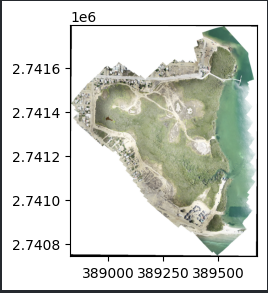
\includegraphics[width=\linewidth,keepaspectratio]{images/mm_drone.png}
      \\
      {\small (a) drone}
    \end{column}
    \begin{column}{0.3\textwidth}
      \centering
      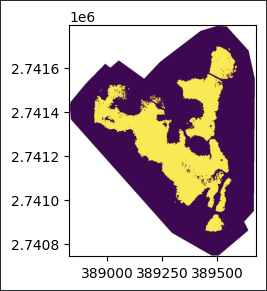
\includegraphics[width=\linewidth,keepaspectratio]{images/mm_label.png}
      \\
      {\small (b) label}
    \end{column}
    \begin{column}{0.3\textwidth}
      \centering
      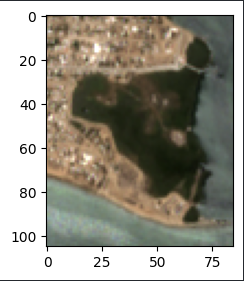
\includegraphics[width=\linewidth,keepaspectratio]{images/mm_sat.png}
      \\
      {\small (c) satellite}
    \end{column}
  \end{columns}
\end{frame}

\begin{frame}{NAIP Data}
    NAIP: High-resolution aerial imagery from the US Department of Agriculture
    \centering
    \begin{figure}
        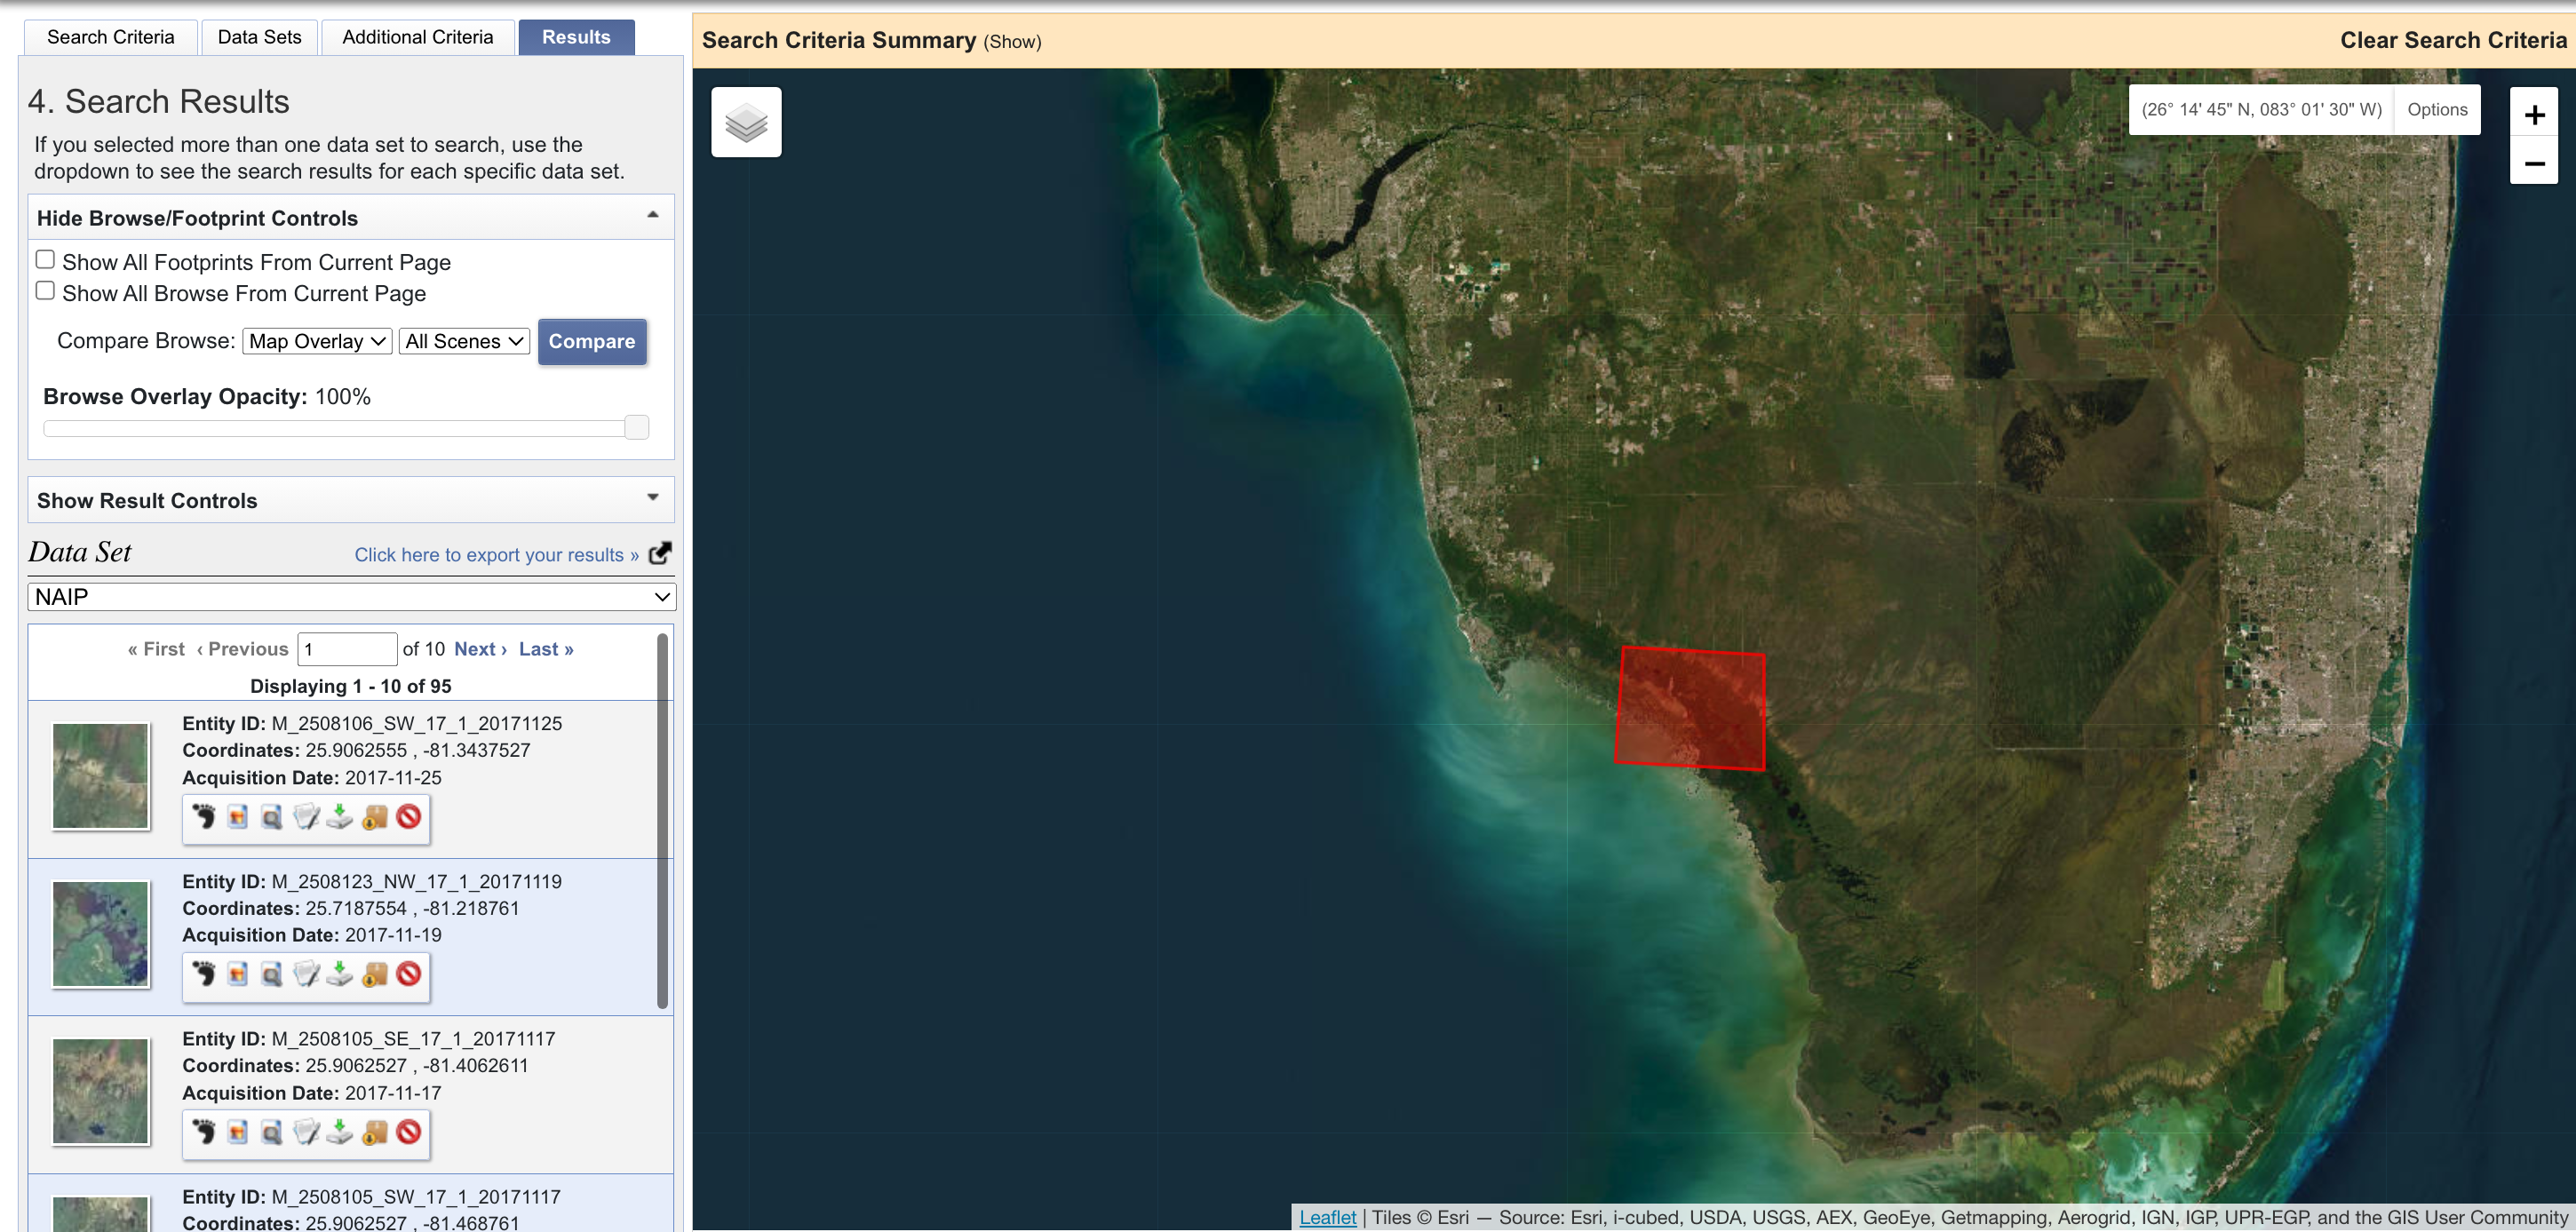
\includegraphics[height=0.7\textheight,width=0.7\textwidth,keepaspectratio]{images/earthexplorer.png}
        \caption{The USGS EarthExplorer interface}
    \end{figure}
\end{frame}

\begin{frame}{In Progress}
    \begin{itemize}
        \item Organize and process other NAS Mexico data
        \item Create tool to mass encode tiled images
    \end{itemize}    
\end{frame}

